\documentclass[twoside]{book}

% Packages required by doxygen
\usepackage{fixltx2e}
\usepackage{calc}
\usepackage{doxygen}
\usepackage[export]{adjustbox} % also loads graphicx
\usepackage{graphicx}
\usepackage[utf8]{inputenc}
\usepackage{makeidx}
\usepackage{multicol}
\usepackage{multirow}
\PassOptionsToPackage{warn}{textcomp}
\usepackage{textcomp}
\usepackage[nointegrals]{wasysym}
\usepackage[table]{xcolor}

% NLS support packages
\usepackage[spanish]{babel}
% Font selection
\usepackage[T1]{fontenc}
\usepackage[scaled=.90]{helvet}
\usepackage{courier}
\usepackage{amssymb}
\usepackage{sectsty}
\renewcommand{\familydefault}{\sfdefault}
\allsectionsfont{%
  \fontseries{bc}\selectfont%
  \color{darkgray}%
}
\renewcommand{\DoxyLabelFont}{%
  \fontseries{bc}\selectfont%
  \color{darkgray}%
}
\newcommand{\+}{\discretionary{\mbox{\scriptsize$\hookleftarrow$}}{}{}}

% Page & text layout
\usepackage{geometry}
\geometry{%
  a4paper,%
  top=2.5cm,%
  bottom=2.5cm,%
  left=2.5cm,%
  right=2.5cm%
}
\tolerance=750
\hfuzz=15pt
\hbadness=750
\setlength{\emergencystretch}{15pt}
\setlength{\parindent}{0cm}
\setlength{\parskip}{3ex plus 2ex minus 2ex}
\makeatletter
\renewcommand{\paragraph}{%
  \@startsection{paragraph}{4}{0ex}{-1.0ex}{1.0ex}{%
    \normalfont\normalsize\bfseries\SS@parafont%
  }%
}
\renewcommand{\subparagraph}{%
  \@startsection{subparagraph}{5}{0ex}{-1.0ex}{1.0ex}{%
    \normalfont\normalsize\bfseries\SS@subparafont%
  }%
}
\makeatother

% Headers & footers
\usepackage{fancyhdr}
\pagestyle{fancyplain}
\fancyhead[LE]{\fancyplain{}{\bfseries\thepage}}
\fancyhead[CE]{\fancyplain{}{}}
\fancyhead[RE]{\fancyplain{}{\bfseries\leftmark}}
\fancyhead[LO]{\fancyplain{}{\bfseries\rightmark}}
\fancyhead[CO]{\fancyplain{}{}}
\fancyhead[RO]{\fancyplain{}{\bfseries\thepage}}
\fancyfoot[LE]{\fancyplain{}{}}
\fancyfoot[CE]{\fancyplain{}{}}
\fancyfoot[RE]{\fancyplain{}{\bfseries\scriptsize Generado por Doxygen }}
\fancyfoot[LO]{\fancyplain{}{\bfseries\scriptsize Generado por Doxygen }}
\fancyfoot[CO]{\fancyplain{}{}}
\fancyfoot[RO]{\fancyplain{}{}}
\renewcommand{\footrulewidth}{0.4pt}
\renewcommand{\chaptermark}[1]{%
  \markboth{#1}{}%
}
\renewcommand{\sectionmark}[1]{%
  \markright{\thesection\ #1}%
}

% Indices & bibliography
\usepackage{natbib}
\usepackage[titles]{tocloft}
\setcounter{tocdepth}{3}
\setcounter{secnumdepth}{5}
\makeindex

% Hyperlinks (required, but should be loaded last)
\usepackage{ifpdf}
\ifpdf
  \usepackage[pdftex,pagebackref=true]{hyperref}
\else
  \usepackage[ps2pdf,pagebackref=true]{hyperref}
\fi
\hypersetup{%
  colorlinks=true,%
  linkcolor=blue,%
  citecolor=blue,%
  unicode%
}

% Custom commands
\newcommand{\clearemptydoublepage}{%
  \newpage{\pagestyle{empty}\cleardoublepage}%
}

\usepackage{caption}
\captionsetup{labelsep=space,justification=centering,font={bf},singlelinecheck=off,skip=4pt,position=top}

%===== C O N T E N T S =====

\begin{document}

% Titlepage & ToC
\hypersetup{pageanchor=false,
             bookmarksnumbered=true,
             pdfencoding=unicode
            }
\pagenumbering{roman}
\begin{titlepage}
\vspace*{7cm}
\begin{center}%
{\Large Banco de Modelos \\[1ex]\large .01 }\\
\vspace*{1cm}
{\large Generado por Doxygen 1.8.11}\\
\end{center}
\end{titlepage}
\clearemptydoublepage
\tableofcontents
\clearemptydoublepage
\pagenumbering{arabic}
\hypersetup{pageanchor=true}

%--- Begin generated contents ---
\chapter{Lanimfe Bank Models}
\label{md_README}
\hypertarget{md_README}{}
This is a simple suit that allows you get some interesting structure factors like Hards Spheere between others.

\subsection*{Getting Started}

There are two ways to use this application one of them is using of the menu guide, you can use this of the following way \subsection*{Easy way}

Open terminal in this source path and execute using the command 
\begin{DoxyCode}
1 ./blds
\end{DoxyCode}
 and follow the structions.

\subsection*{A more advanced way}

This program contains severals options that you can use for interact with the structures factors and their results.

For example if you type 
\begin{DoxyCode}
1 ./blds HS
\end{DoxyCode}
 the process for calculate the Hard Spheere structure factor executes.

{\bfseries Here are the differents options that you can execute with this programm.}


\begin{DoxyCode}
1 ./blds HS
\end{DoxyCode}
 {\itshape Executes the process for calculate the Hard Sphere structure factor}


\begin{DoxyCode}
1 ./blds SS
\end{DoxyCode}
 {\itshape Executes the process for calculate the Soft Sphere structure factor}


\begin{DoxyCode}
1 ./blds Yuk
\end{DoxyCode}
 {\itshape Executes the process for calculate the Yukawa 3D structure factor}


\begin{DoxyCode}
1 ./blds plot HS
\end{DoxyCode}
 {\itshape Plot the Data of Hard Spheere Structure Factor}


\begin{DoxyCode}
1 ./blds plot SS
\end{DoxyCode}
 {\itshape Plot the Data of Soft Spheere Structure Factor}


\begin{DoxyCode}
1 ./blds plot Yuk
\end{DoxyCode}
 {\itshape Plot the Data of Yukawa 3D Structure Factor}


\begin{DoxyCode}
1 ./blds print HS
\end{DoxyCode}
 {\itshape Print the Data of Hard Spheere Structure Factor}


\begin{DoxyCode}
1 ./blds print SS
\end{DoxyCode}
 {\itshape Print the Data of Soft Spheere Structure Factor}


\begin{DoxyCode}
1 ./blds print Yuk
\end{DoxyCode}
 {\itshape Print the Data of Yukawa 3D Structure Factor}


\begin{DoxyCode}
1 ./blds dir
\end{DoxyCode}

\begin{DoxyItemize}
\item List all the files avaible of the structures factors$\ast$
\end{DoxyItemize}

\subsection*{Special Notes}

You can edit certains properties about the structures factors like volumen fractions if you edit the files of the config directory. 
\chapter{Índice de clases}
\section{Class List}
Here are the classes, structs, unions and interfaces with brief descriptions\+:\begin{DoxyCompactList}
\item\contentsline{section}{\hyperlink{class_file___manage}{File\+\_\+\+Manage} \\*Clase para el manejo de archivos }{\pageref{class_file___manage}}{}
\item\contentsline{section}{\hyperlink{class_hard___sphere___dynamic}{Hard\+\_\+\+Sphere\+\_\+\+Dynamic} }{\pageref{class_hard___sphere___dynamic}}{}
\item\contentsline{section}{\hyperlink{class_hard___sphere___mono}{Hard\+\_\+\+Sphere\+\_\+\+Mono} \\*Realiza todas las operaciones para el calculo de Sk de esfera dura }{\pageref{class_hard___sphere___mono}}{}
\item\contentsline{section}{\hyperlink{class_static___variables}{Static\+\_\+\+Variables} }{\pageref{class_static___variables}}{}
\item\contentsline{section}{\hyperlink{class_sys___variables}{Sys\+\_\+\+Variables} }{\pageref{class_sys___variables}}{}
\end{DoxyCompactList}

\chapter{Indice de archivos}
\section{Lista de archivos}
Lista de todos los archivos documentados y con descripciones breves\+:\begin{DoxyCompactList}
\item\contentsline{section}{\hyperlink{main_8cpp}{main.\+cpp} }{\pageref{main_8cpp}}{}
\item\contentsline{section}{headers/{\bfseries file\+\_\+manage.\+hpp} }{\pageref{file__manage_8hpp}}{}
\item\contentsline{section}{headers/{\bfseries H\+P\+P\+\_\+headers.\+hpp} }{\pageref{_h_p_p__headers_8hpp}}{}
\item\contentsline{section}{headers/{\bfseries main.\+hpp} }{\pageref{main_8hpp}}{}
\item\contentsline{section}{headers/{\bfseries menu\+\_\+things.\+hpp} }{\pageref{menu__things_8hpp}}{}
\end{DoxyCompactList}

\chapter{Documentación de las clases}
\hypertarget{class_file___manage}{}\section{Referencia de la Clase File\+\_\+\+Manage}
\label{class_file___manage}\index{File\+\_\+\+Manage@{File\+\_\+\+Manage}}


Clase que se encarga de toda las funciones que tienen que ver con la manipulacion de archivos, ademas de la interaccion del sistema de archivos del host.  




{\ttfamily \#include $<$file\+\_\+manage.\+hpp$>$}

\subsection*{Métodos públicos}
\begin{DoxyCompactItemize}
\item 
\hyperlink{class_file___manage_abc8dc9e06400e1b1e67a8d9dddef4393}{File\+\_\+\+Manage} ()
\item 
\hyperlink{class_file___manage_a0315b0bb47c3572e17978b367aef66b9}{File\+\_\+\+Manage} (const std\+::string \&str, bool truncate)
\item 
\hyperlink{class_file___manage_a304e6be6ea118b79bf9aa2bf6fad5523}{$\sim$\+File\+\_\+\+Manage} ()
\item 
void \hyperlink{class_file___manage_a994b1789f2e06c194cd9e50c708197cd}{save\+\_\+sk} (double $\ast$sk, double $\ast$k, int Kpoints, int species)
\item 
bool {\bfseries read\+\_\+\+Sk} ()\hypertarget{class_file___manage_a1e38c35a55c0ed0d5323a93e8aa2ef97}{}\label{class_file___manage_a1e38c35a55c0ed0d5323a93e8aa2ef97}

\item 
void {\bfseries read\+\_\+file\+\_\+line\+\_\+by\+\_\+line\+\_\+p} ()\hypertarget{class_file___manage_a92234a6c1b0ee752da82a10dc8c1f67c}{}\label{class_file___manage_a92234a6c1b0ee752da82a10dc8c1f67c}

\item 
std\+::vector$<$ std\+::string $>$ \hyperlink{class_file___manage_aa433eb719c0e2aca12ccf7318c88fd18}{read\+\_\+file\+\_\+line\+\_\+by\+\_\+line\+\_\+g} (std\+::string)
\item 
void \hyperlink{class_file___manage_a4fad3d9f394f5fd1f6d8a3accec9c4d1}{set\+\_\+date\+\_\+\+F\+I\+L\+E\+\_\+from\+\_\+\+Options\+\_\+file} ()
\item 
void \hyperlink{class_file___manage_a43a37464905930b06edbf0c4f54f7535}{create\+\_\+directory} (const char $\ast$dir\+\_\+name\mbox{[}$\,$\mbox{]})
\item 
void \hyperlink{class_file___manage_a3b93465cf17542be8ad7003f8924e12b}{Add\+\_\+a\+\_\+\+File\+\_\+to\+\_\+\+Directory\+\_\+\+Date} (const char dir\+\_\+name\mbox{[}$\,$\mbox{]})
\item 
void {\bfseries save\+\_\+\+Sk\+\_\+\+S\+S\+Phere} (int n\+Kas, double phi, double deltaK, double \+\_\+dss, double $\ast$sk)\hypertarget{class_file___manage_a37663503715d54409a9b7bf661971720}{}\label{class_file___manage_a37663503715d54409a9b7bf661971720}

\item 
char $\ast$ {\bfseries get\+\_\+date} ()\hypertarget{class_file___manage_a369015860dcc9bc16e5445f967e44d9d}{}\label{class_file___manage_a369015860dcc9bc16e5445f967e44d9d}

\item 
std\+::vector$<$ std\+::string $>$ {\bfseries my\+\_\+split} (const std\+::string \&str, char delim)\hypertarget{class_file___manage_af9137339f79aaac3f9e5aa398364b625}{}\label{class_file___manage_af9137339f79aaac3f9e5aa398364b625}

\item 
std\+::vector$<$ std\+::string $>$ \& {\bfseries split} (const std\+::string \&s, char delim, std\+::vector$<$ std\+::string $>$ \&elems)\hypertarget{class_file___manage_a1611614dd81969a1722a91178e5b4787}{}\label{class_file___manage_a1611614dd81969a1722a91178e5b4787}

\item 
std\+::vector$<$ std\+::string $>$ {\bfseries get\+\_\+just\+\_\+numbrs} (std\+::vector$<$ std\+::string $>$lines)\hypertarget{class_file___manage_afc1e5a4741aab41c324cea922cc975fc}{}\label{class_file___manage_afc1e5a4741aab41c324cea922cc975fc}

\item 
void {\bfseries save\+\_\+\+S\+K\+\_\+\+M\+O\+NO} (double $\ast$sk, double $\ast$k, int Kpoints)\hypertarget{class_file___manage_abb0a79ecc1c74608831544a979e3f931}{}\label{class_file___manage_abb0a79ecc1c74608831544a979e3f931}

\item 
void {\bfseries print\+\_\+file} (const std\+::string \&str)\hypertarget{class_file___manage_ab8161cc5685ac0347078f62dd816a4bc}{}\label{class_file___manage_ab8161cc5685ac0347078f62dd816a4bc}

\item 
int {\bfseries print\+\_\+directory} ()\hypertarget{class_file___manage_ada7d3f8c329658f0a234f87c194ca0cb}{}\label{class_file___manage_ada7d3f8c329658f0a234f87c194ca0cb}

\end{DoxyCompactItemize}
\subsection*{Atributos protegidos}
\begin{DoxyCompactItemize}
\item 
std\+::string \hyperlink{class_file___manage_a34a7f1a17609e115811efc140a07a018}{file\+\_\+name}
\item 
bool \hyperlink{class_file___manage_a598d159493673c0864cd0873816f33a8}{truncate\+\_\+file}
\item 
std\+::ofstream \hyperlink{class_file___manage_ab1ba9c8b82239cec993eff15781ec0be}{outfile}
\item 
std\+::ifstream \hyperlink{class_file___manage_a8c530b8325a65e290ea3db405f91234a}{infile}
\item 
char \hyperlink{class_file___manage_a8bf6f9762a78137d34b859a86d595844}{\+\_\+date} \mbox{[}50\mbox{]}
\item 
char {\bfseries \+\_\+directory\+\_\+name} \mbox{[}100\mbox{]}\hypertarget{class_file___manage_a0c1a126aa8ac02089aa1568b958aebb8}{}\label{class_file___manage_a0c1a126aa8ac02089aa1568b958aebb8}

\item 
F\+I\+LE $\ast$ {\bfseries \+\_\+directory}\hypertarget{class_file___manage_a418a904721b58fd5f506cc8b6fe155c9}{}\label{class_file___manage_a418a904721b58fd5f506cc8b6fe155c9}

\end{DoxyCompactItemize}


\subsection{Descripción detallada}
Clase que se encarga de toda las funciones que tienen que ver con la manipulacion de archivos, ademas de la interaccion del sistema de archivos del host. 

\subsection{Documentación del constructor y destructor}
\index{File\+\_\+\+Manage@{File\+\_\+\+Manage}!File\+\_\+\+Manage@{File\+\_\+\+Manage}}
\index{File\+\_\+\+Manage@{File\+\_\+\+Manage}!File\+\_\+\+Manage@{File\+\_\+\+Manage}}
\subsubsection[{\texorpdfstring{File\+\_\+\+Manage()}{File_Manage()}}]{\setlength{\rightskip}{0pt plus 5cm}File\+\_\+\+Manage\+::\+File\+\_\+\+Manage (
\begin{DoxyParamCaption}
{}
\end{DoxyParamCaption}
)}\hypertarget{class_file___manage_abc8dc9e06400e1b1e67a8d9dddef4393}{}\label{class_file___manage_abc8dc9e06400e1b1e67a8d9dddef4393}
brief Constructor default de la clase. \index{File\+\_\+\+Manage@{File\+\_\+\+Manage}!File\+\_\+\+Manage@{File\+\_\+\+Manage}}
\index{File\+\_\+\+Manage@{File\+\_\+\+Manage}!File\+\_\+\+Manage@{File\+\_\+\+Manage}}
\subsubsection[{\texorpdfstring{File\+\_\+\+Manage(const std\+::string \&str, bool truncate)}{File_Manage(const std::string &str, bool truncate)}}]{\setlength{\rightskip}{0pt plus 5cm}File\+\_\+\+Manage\+::\+File\+\_\+\+Manage (
\begin{DoxyParamCaption}
\item[{const std\+::string \&}]{str, }
\item[{bool}]{truncate}
\end{DoxyParamCaption}
)}\hypertarget{class_file___manage_a0315b0bb47c3572e17978b367aef66b9}{}\label{class_file___manage_a0315b0bb47c3572e17978b367aef66b9}
Crea un archivo con el nombre especificado, ademas de indicar si este mismo desea truncarlo o no. 
\begin{DoxyParams}{Parámetros}
{\em str} & nombre del archivo, este incluye la ruta del mismo. \\
\hline
{\em truncate} & simple bandera para indicar si desea que este sea truncado o no. \\
\hline
\end{DoxyParams}
\index{File\+\_\+\+Manage@{File\+\_\+\+Manage}!````~File\+\_\+\+Manage@{$\sim$\+File\+\_\+\+Manage}}
\index{````~File\+\_\+\+Manage@{$\sim$\+File\+\_\+\+Manage}!File\+\_\+\+Manage@{File\+\_\+\+Manage}}
\subsubsection[{\texorpdfstring{$\sim$\+File\+\_\+\+Manage()}{~File_Manage()}}]{\setlength{\rightskip}{0pt plus 5cm}File\+\_\+\+Manage\+::$\sim$\+File\+\_\+\+Manage (
\begin{DoxyParamCaption}
{}
\end{DoxyParamCaption}
)}\hypertarget{class_file___manage_a304e6be6ea118b79bf9aa2bf6fad5523}{}\label{class_file___manage_a304e6be6ea118b79bf9aa2bf6fad5523}
Destructor default de la clase. 

\subsection{Documentación de las funciones miembro}
\index{File\+\_\+\+Manage@{File\+\_\+\+Manage}!Add\+\_\+a\+\_\+\+File\+\_\+to\+\_\+\+Directory\+\_\+\+Date@{Add\+\_\+a\+\_\+\+File\+\_\+to\+\_\+\+Directory\+\_\+\+Date}}
\index{Add\+\_\+a\+\_\+\+File\+\_\+to\+\_\+\+Directory\+\_\+\+Date@{Add\+\_\+a\+\_\+\+File\+\_\+to\+\_\+\+Directory\+\_\+\+Date}!File\+\_\+\+Manage@{File\+\_\+\+Manage}}
\subsubsection[{\texorpdfstring{Add\+\_\+a\+\_\+\+File\+\_\+to\+\_\+\+Directory\+\_\+\+Date(const char dir\+\_\+name[])}{Add_a_File_to_Directory_Date(const char dir_name[])}}]{\setlength{\rightskip}{0pt plus 5cm}void File\+\_\+\+Manage\+::\+Add\+\_\+a\+\_\+\+File\+\_\+to\+\_\+\+Directory\+\_\+\+Date (
\begin{DoxyParamCaption}
\item[{const char}]{file\+\_\+name\mbox{[}$\,$\mbox{]}}
\end{DoxyParamCaption}
)}\hypertarget{class_file___manage_a3b93465cf17542be8ad7003f8924e12b}{}\label{class_file___manage_a3b93465cf17542be8ad7003f8924e12b}
Add a file to a directory with the name in \+\_\+date \index{File\+\_\+\+Manage@{File\+\_\+\+Manage}!create\+\_\+directory@{create\+\_\+directory}}
\index{create\+\_\+directory@{create\+\_\+directory}!File\+\_\+\+Manage@{File\+\_\+\+Manage}}
\subsubsection[{\texorpdfstring{create\+\_\+directory(const char $\ast$dir\+\_\+name[])}{create_directory(const char *dir_name[])}}]{\setlength{\rightskip}{0pt plus 5cm}void File\+\_\+\+Manage\+::create\+\_\+directory (
\begin{DoxyParamCaption}
\item[{const char $\ast$}]{dir\+\_\+name\mbox{[}$\,$\mbox{]}}
\end{DoxyParamCaption}
)}\hypertarget{class_file___manage_a43a37464905930b06edbf0c4f54f7535}{}\label{class_file___manage_a43a37464905930b06edbf0c4f54f7535}
Just create a simple normal directory. 
\begin{DoxyParams}{Parámetros}
{\em dir\+\_\+name} & -\/ Is the name of the directory. \\
\hline
\end{DoxyParams}
\index{File\+\_\+\+Manage@{File\+\_\+\+Manage}!read\+\_\+file\+\_\+line\+\_\+by\+\_\+line\+\_\+g@{read\+\_\+file\+\_\+line\+\_\+by\+\_\+line\+\_\+g}}
\index{read\+\_\+file\+\_\+line\+\_\+by\+\_\+line\+\_\+g@{read\+\_\+file\+\_\+line\+\_\+by\+\_\+line\+\_\+g}!File\+\_\+\+Manage@{File\+\_\+\+Manage}}
\subsubsection[{\texorpdfstring{read\+\_\+file\+\_\+line\+\_\+by\+\_\+line\+\_\+g(std\+::string)}{read_file_line_by_line_g(std::string)}}]{\setlength{\rightskip}{0pt plus 5cm}std\+::vector$<$ std\+::string $>$ File\+\_\+\+Manage\+::read\+\_\+file\+\_\+line\+\_\+by\+\_\+line\+\_\+g (
\begin{DoxyParamCaption}
\item[{std\+::string}]{str}
\end{DoxyParamCaption}
)}\hypertarget{class_file___manage_aa433eb719c0e2aca12ccf7318c88fd18}{}\label{class_file___manage_aa433eb719c0e2aca12ccf7318c88fd18}
Read a text file line by line, load this information in a vector and return it. \index{File\+\_\+\+Manage@{File\+\_\+\+Manage}!save\+\_\+sk@{save\+\_\+sk}}
\index{save\+\_\+sk@{save\+\_\+sk}!File\+\_\+\+Manage@{File\+\_\+\+Manage}}
\subsubsection[{\texorpdfstring{save\+\_\+sk(double $\ast$sk, double $\ast$k, int Kpoints, int species)}{save_sk(double *sk, double *k, int Kpoints, int species)}}]{\setlength{\rightskip}{0pt plus 5cm}void File\+\_\+\+Manage\+::save\+\_\+sk (
\begin{DoxyParamCaption}
\item[{double $\ast$}]{sk, }
\item[{double $\ast$}]{k, }
\item[{int}]{Kpoints, }
\item[{int}]{species}
\end{DoxyParamCaption}
)}\hypertarget{class_file___manage_a994b1789f2e06c194cd9e50c708197cd}{}\label{class_file___manage_a994b1789f2e06c194cd9e50c708197cd}
Guarda el factor de estructura para esfera dura. 
\begin{DoxyParams}{Parámetros}
{\em sk} & arreglo que contiene los datos del factor de estructura. \\
\hline
{\em k} & arreglo que contiene datos relativos al factor de estructura. \\
\hline
{\em kpoints} & numero de puntos que contiene el factor de estructura. \\
\hline
{\em species} & numero de especies en el sistema. \\
\hline
\end{DoxyParams}
\index{File\+\_\+\+Manage@{File\+\_\+\+Manage}!set\+\_\+date\+\_\+\+F\+I\+L\+E\+\_\+from\+\_\+\+Options\+\_\+file@{set\+\_\+date\+\_\+\+F\+I\+L\+E\+\_\+from\+\_\+\+Options\+\_\+file}}
\index{set\+\_\+date\+\_\+\+F\+I\+L\+E\+\_\+from\+\_\+\+Options\+\_\+file@{set\+\_\+date\+\_\+\+F\+I\+L\+E\+\_\+from\+\_\+\+Options\+\_\+file}!File\+\_\+\+Manage@{File\+\_\+\+Manage}}
\subsubsection[{\texorpdfstring{set\+\_\+date\+\_\+\+F\+I\+L\+E\+\_\+from\+\_\+\+Options\+\_\+file()}{set_date_FILE_from_Options_file()}}]{\setlength{\rightskip}{0pt plus 5cm}void File\+\_\+\+Manage\+::set\+\_\+date\+\_\+\+F\+I\+L\+E\+\_\+from\+\_\+\+Options\+\_\+file (
\begin{DoxyParamCaption}
{}
\end{DoxyParamCaption}
)}\hypertarget{class_file___manage_a4fad3d9f394f5fd1f6d8a3accec9c4d1}{}\label{class_file___manage_a4fad3d9f394f5fd1f6d8a3accec9c4d1}
Get the current date and time and set this in the \+\_\+date array. this must to read the options file for read some properties as like final tempeture, incial tempeture between others. T\+H\+IS IS C\+AN C\+H\+A\+N\+GE IS A H\+O\+R\+R\+I\+B\+LE S\+N\+I\+P\+ET C\+O\+DE 

\subsection{Documentación de los datos miembro}
\index{File\+\_\+\+Manage@{File\+\_\+\+Manage}!\+\_\+date@{\+\_\+date}}
\index{\+\_\+date@{\+\_\+date}!File\+\_\+\+Manage@{File\+\_\+\+Manage}}
\subsubsection[{\texorpdfstring{\+\_\+date}{_date}}]{\setlength{\rightskip}{0pt plus 5cm}char File\+\_\+\+Manage\+::\+\_\+date\mbox{[}50\mbox{]}\hspace{0.3cm}{\ttfamily [protected]}}\hypertarget{class_file___manage_a8bf6f9762a78137d34b859a86d595844}{}\label{class_file___manage_a8bf6f9762a78137d34b859a86d595844}
Para guardar la fecha actual. \index{File\+\_\+\+Manage@{File\+\_\+\+Manage}!file\+\_\+name@{file\+\_\+name}}
\index{file\+\_\+name@{file\+\_\+name}!File\+\_\+\+Manage@{File\+\_\+\+Manage}}
\subsubsection[{\texorpdfstring{file\+\_\+name}{file_name}}]{\setlength{\rightskip}{0pt plus 5cm}std\+::string File\+\_\+\+Manage\+::file\+\_\+name\hspace{0.3cm}{\ttfamily [protected]}}\hypertarget{class_file___manage_a34a7f1a17609e115811efc140a07a018}{}\label{class_file___manage_a34a7f1a17609e115811efc140a07a018}
Nombre del archivo, este ademas incluye la ruta del mismo \index{File\+\_\+\+Manage@{File\+\_\+\+Manage}!infile@{infile}}
\index{infile@{infile}!File\+\_\+\+Manage@{File\+\_\+\+Manage}}
\subsubsection[{\texorpdfstring{infile}{infile}}]{\setlength{\rightskip}{0pt plus 5cm}std \+:: ifstream File\+\_\+\+Manage\+::infile\hspace{0.3cm}{\ttfamily [protected]}}\hypertarget{class_file___manage_a8c530b8325a65e290ea3db405f91234a}{}\label{class_file___manage_a8c530b8325a65e290ea3db405f91234a}
Para leer archivos. \index{File\+\_\+\+Manage@{File\+\_\+\+Manage}!outfile@{outfile}}
\index{outfile@{outfile}!File\+\_\+\+Manage@{File\+\_\+\+Manage}}
\subsubsection[{\texorpdfstring{outfile}{outfile}}]{\setlength{\rightskip}{0pt plus 5cm}std \+:: ofstream File\+\_\+\+Manage\+::outfile\hspace{0.3cm}{\ttfamily [protected]}}\hypertarget{class_file___manage_ab1ba9c8b82239cec993eff15781ec0be}{}\label{class_file___manage_ab1ba9c8b82239cec993eff15781ec0be}
Para escribir archivos. \index{File\+\_\+\+Manage@{File\+\_\+\+Manage}!truncate\+\_\+file@{truncate\+\_\+file}}
\index{truncate\+\_\+file@{truncate\+\_\+file}!File\+\_\+\+Manage@{File\+\_\+\+Manage}}
\subsubsection[{\texorpdfstring{truncate\+\_\+file}{truncate_file}}]{\setlength{\rightskip}{0pt plus 5cm}bool File\+\_\+\+Manage\+::truncate\+\_\+file\hspace{0.3cm}{\ttfamily [protected]}}\hypertarget{class_file___manage_a598d159493673c0864cd0873816f33a8}{}\label{class_file___manage_a598d159493673c0864cd0873816f33a8}
Indica si el archivo se tiene que truncar o no. 

La documentación para esta clase fue generada a partir de los siguientes ficheros\+:\begin{DoxyCompactItemize}
\item 
headers/file\+\_\+manage.\+hpp\item 
file\+\_\+manage.\+cpp\end{DoxyCompactItemize}

\hypertarget{class_menu___class}{}\section{Referencia de la Clase Menu\+\_\+\+Class}
\label{class_menu___class}\index{Menu\+\_\+\+Class@{Menu\+\_\+\+Class}}
\subsection*{Métodos públicos}
\begin{DoxyCompactItemize}
\item 
void {\bfseries print\+\_\+preface} ()\hypertarget{class_menu___class_ac15bd27926bcdad8dfb6415472aee4bf}{}\label{class_menu___class_ac15bd27926bcdad8dfb6415472aee4bf}

\item 
void {\bfseries print\+\_\+help} ()\hypertarget{class_menu___class_a228296373587bc325379923221e5abf4}{}\label{class_menu___class_a228296373587bc325379923221e5abf4}

\item 
int {\bfseries print\+\_\+directory} ()\hypertarget{class_menu___class_a9c5983a219395bb87d032ddfb1425873}{}\label{class_menu___class_a9c5983a219395bb87d032ddfb1425873}

\item 
void {\bfseries print\+\_\+main\+\_\+loop\+\_\+menu} ()\hypertarget{class_menu___class_ae28cf78b5be2bea670ac24fbe89920df}{}\label{class_menu___class_ae28cf78b5be2bea670ac24fbe89920df}

\item 
void {\bfseries print\+\_\+options} (const std\+::string \&str)\hypertarget{class_menu___class_a97f33152f31c98c3cc967f23dd18fcfd}{}\label{class_menu___class_a97f33152f31c98c3cc967f23dd18fcfd}

\end{DoxyCompactItemize}


La documentación para esta clase fue generada a partir de los siguientes ficheros\+:\begin{DoxyCompactItemize}
\item 
headers/menu\+\_\+things.\+hpp\item 
menu\+\_\+things.\+cpp\end{DoxyCompactItemize}

\chapter{Documentación de archivos}
\hypertarget{main_8cpp}{}\section{main.\+cpp File Reference}
\label{main_8cpp}\index{main.\+cpp@{main.\+cpp}}
{\ttfamily \#include $<$hard\+\_\+sphere\+\_\+dynamics.\+hpp$>$}\\*
{\ttfamily \#include $<$iostream$>$}\\*
{\ttfamily \#include $<$stdio.\+h$>$}\\*
{\ttfamily \#include $<$cstdlib$>$}\\*
Include dependency graph for main.\+cpp\+:\nopagebreak
\begin{figure}[H]
\begin{center}
\leavevmode
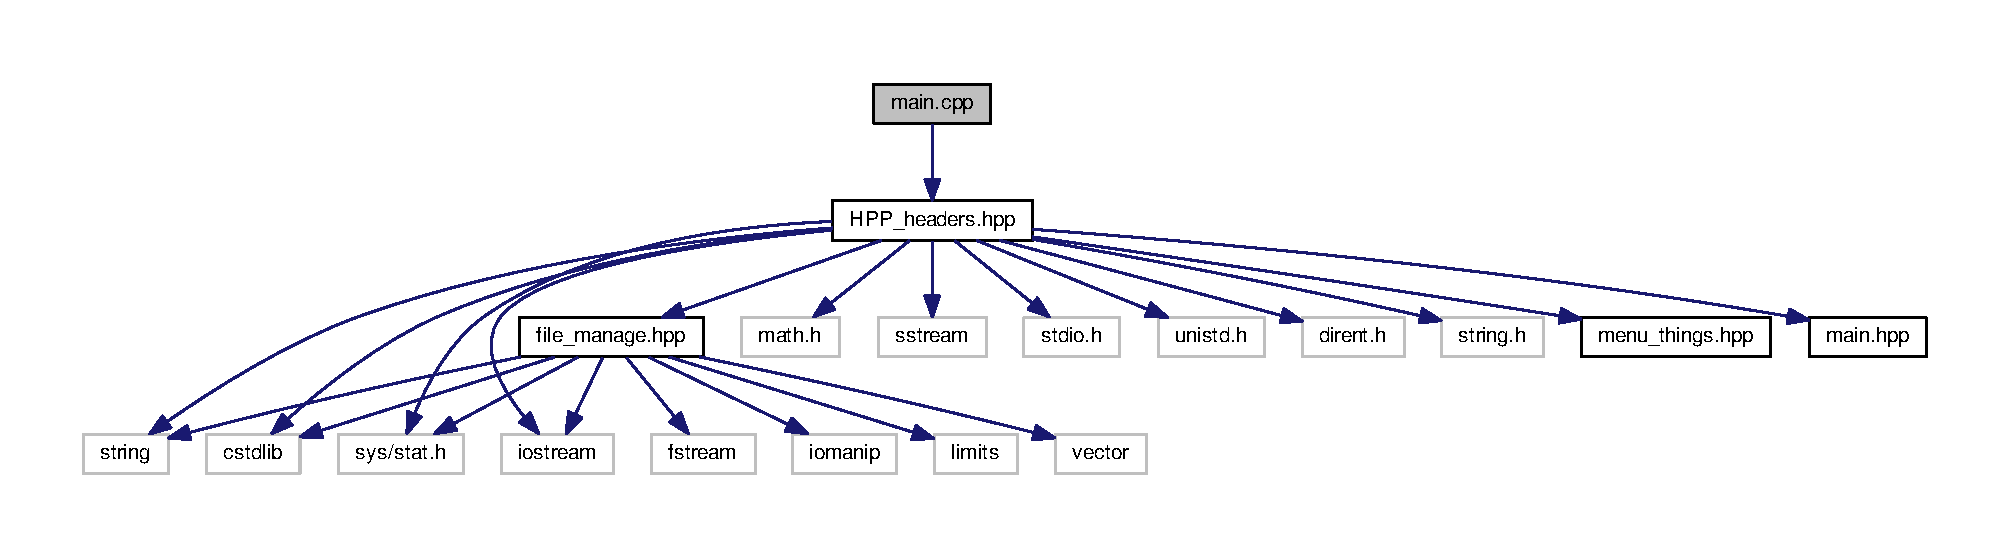
\includegraphics[width=350pt]{main_8cpp__incl}
\end{center}
\end{figure}
\subsection*{Functions}
\begin{DoxyCompactItemize}
\item 
int \hyperlink{main_8cpp_ac0f2228420376f4db7e1274f2b41667c}{main} (int argc, const char $\ast$argv\mbox{[}$\,$\mbox{]})
\end{DoxyCompactItemize}


\subsection{Function Documentation}
\index{main.\+cpp@{main.\+cpp}!main@{main}}
\index{main@{main}!main.\+cpp@{main.\+cpp}}
\subsubsection[{\texorpdfstring{main(int argc, const char $\ast$argv[])}{main(int argc, const char *argv[])}}]{\setlength{\rightskip}{0pt plus 5cm}int main (
\begin{DoxyParamCaption}
\item[{int}]{argc, }
\item[{const char $\ast$}]{argv\mbox{[}$\,$\mbox{]}}
\end{DoxyParamCaption}
)}\hypertarget{main_8cpp_ac0f2228420376f4db7e1274f2b41667c}{}\label{main_8cpp_ac0f2228420376f4db7e1274f2b41667c}
Funcion principal de donde parte la ejecucion para el calculo del factor de estructura para para esfera dura. 

Definition at line 11 of file main.\+cpp.


%--- End generated contents ---

% Index
\backmatter
\newpage
\phantomsection
\clearemptydoublepage
\addcontentsline{toc}{chapter}{Índice}
\printindex

\end{document}
